\documentclass[aspectratio=169,10pt]{beamer}
\usetheme{Madrid}
\usepackage[T1]{fontenc}

\usepackage{fancybox,graphicx,hyperref,url}
\usepackage{tikz}
\usetikzlibrary{shapes,arrows}
\usetikzlibrary{positioning}
\usepackage{booktabs}
\usepackage{enumitem}

\usepackage{listings}
\usepackage{pdfpages}
\usepackage{lstautogobble}

\usepackage[listings,skins,breakable,xparse]{tcolorbox}
\tcbuselibrary{theorems}
\tcbset{highlight math/.append style={boxrule=0pt,
                                      frame hidden,
                                      colback=yellow!40!white,
                                      sharp corners}}

\usepackage{xpatch}
\usepackage{xcolor}
\usepackage{realboxes}
\usetikzlibrary{fit}
\usetikzlibrary{shadings}
\usetikzlibrary{shapes.arrows,shadows.blur}

\pgfdeclarefunctionalshading{Hermite-Gaussian modes}{\pgfpoint{-25bp}{-25bp}}{\pgfpoint{25bp}{25bp}}{}{
    10 atan sin 1000 mul cos 1 add
    exch
    10 atan sin 1000 mul cos 1 add
    mul 4 div
    dup dup
}

\makeatletter
\xpretocmd\lstinline{\Colorbox{yellow!10!white}\bgroup\appto\lst@DeInit{\egroup}}{}{}
\makeatother

\definecolor{my_red}{RGB}{128, 0, 0}

\lstset{captionpos=b}
\lstset{numberbychapter=false}
\lstset{autogobble}
% \lstset{breaklines=true}

\usepackage{tikz}
\usepackage{subcaption}
\usetikzlibrary{calc, chains, decorations.pathmorphing}
\usetikzlibrary{shapes,arrows,backgrounds}
\usetikzlibrary{positioning,fit,shapes.geometric,shapes}

\setbeamercovered{transparent}

\setlistdepth{9}
\setlist[itemize,1]{label=$\bullet$}
\setlist[itemize,2]{label=$\bullet$}
\setlist[itemize,3]{label=$\bullet$}
\setlist[itemize,4]{label=$\bullet$}
\setlist[itemize,5]{label=$\bullet$}
\setlist[itemize,6]{label=$\bullet$}
\setlist[itemize,7]{label=$\bullet$}
\setlist[itemize,8]{label=$\bullet$}
\setlist[itemize,9]{label=$\bullet$}
\renewlist{itemize}{itemize}{9}

\setlist[enumerate,1]{label=$\arabic*.$}
\setlist[enumerate,2]{label=$\alph*.$}
\setlist[enumerate,3]{label=$\roman*.$}
\setlist[enumerate,4]{label=$\arabic*.$}
\setlist[enumerate,5]{label=$\alpha*$}
\setlist[enumerate,6]{label=$\roman*.$}
\setlist[enumerate,7]{label=$\arabic*.$}
\setlist[enumerate,8]{label=$\alph*.$}
\setlist[enumerate,9]{label=$\roman*.$}
\renewlist{enumerate}{enumerate}{9}

\AtBeginSection[]{
  \begin{frame}[noframenumbering]
    \vfill
    \centering
    \begin{beamercolorbox}[sep=8pt,center,shadow=true,rounded=true]{title}
      \usebeamerfont{title}\insertsectionhead\par%
    \end{beamercolorbox}
    \vfill
  \end{frame}
}

\title[Nondeterministic Asynchronous Dataflow in Isabelle/HOL]{Nondeterministic Asynchronous Dataflow in Isabelle/HOL}

\author[Rafael, Laouen and Dmitriy]{
  Rafael Castro G. Silva, Laouen Fernet and  Dmitriy Traytel\\\medskip
  {\small \url{rasi@di.ku.dk}}}

\date{14/05/2025}

% change title (done)
% (co)datatypes -> codatatypes (done)
% while_option from HOL library (done)
% coindtive principle -> coinduction principle (done)
% remove next step slide, andd as a bullet (done)
% explain slice in more detail (done)
% mention selectors in llist slide, drop lmap, drop lset (done)
% move count operator example to slide that introduce op type (done)
% modeling lazy list processors which do not care about time (done)
% reduce Corecursion is like recursion line (done)
% why partial order? mention timely dataflow (done)
% explain what incremental, and set expectation for example (done)
% move arrows (done)
% Change push to out, done to out (done)
% put star footnote on op type saying it is simplified compare to the paper, also in the composition lemma (done)
% write the lapp lemma about lfinite (done)
% show coinduction principle for llist (done)
% add link llist afp (done)
% on produce slide, metion lshift as friend (point to freinds with benefits paper) (done)
% justify the compositional reasoning with lines of code for each building block (done)
% slide about tecnicques used, coinduction principles, friends, reasoning up to friends, generalization using skip_op, combining coinduction and induction, coinduction up to congruence for coinductive predicates, say our paper is more detailed in these topics
%
% add definition of batch_op, and all 4 properties

\institute[UCPH]{
  Department of Computer Science \\
  University of Copenhagen}

\begin{document}
\setbeamercovered{invisible}
% \setbeamercovered{dynamic}

\begin{frame}
  \titlepage

\end{frame}
\section{Motivation}
\begin{frame}[fragile]
  \frametitle{Motivation}
  \begin{block}{Context:}
  \begin{itemize}
    \item Stream Processing: programs that compute (possibly) unbounded sequences of data (streams)
    \item A common problem in the industry
    \item Frameworks:\\ Apache Flink, Apache Samza, Apache Spark, Google Cloud Dataflow, and Timely Dataflow
          \begin{figure}
            \centering
            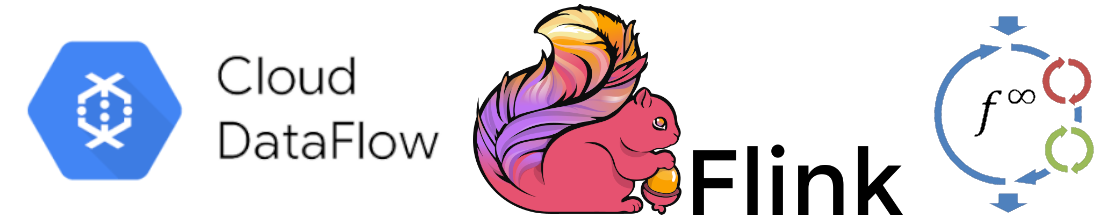
\includegraphics[scale=0.1]{all}
          \end{figure}
    \item Why use frameworks?
          \begin{itemize}
            \item Highly Parallel
            \item Low latency (output as soon as possible)
            \item Incremental computing (re-uses previous computations)
          \end{itemize}
  \end{itemize}
  \pause
  \end{block}
  \begin{block}{Our goal:}
    Mechanically Verify Timely Dataflow algorithms
  \end{block}

\end{frame}

\section{A Good Foundation}

\begin{frame}[fragile]
  \frametitle{A Good Foundation}
  \begin{columns}
    \begin{column}{.35\textwidth}
      \begin{figure}
        \centering
        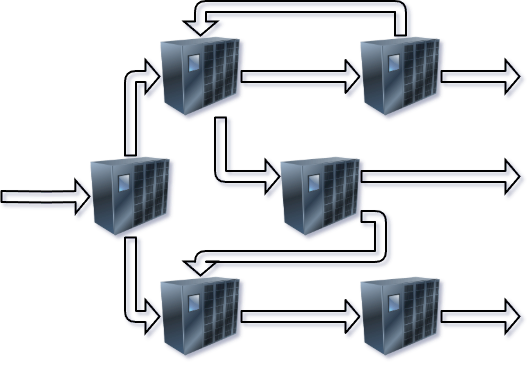
\includegraphics[width=1\textwidth]{network.png}
      \end{figure}
    \end{column}
    \begin{column}{.65\textwidth}
      \begin{itemize}
        \item Nondeterministic Asynchronous Dataflow
              \begin{itemize}
                \pause
                \item Dataflow: Directed graph of interconnected operators
                \pause
                \item Asynchronous:
                      \begin{itemize}
                        \item Operators execute independently:\\ processes without an orchestrator
                        \item Operators can freely communicate with the network (read/write); do silent computation steps
                        \item Networks are unbounded FIFO queues
                      \end{itemize}
                \pause
                \item Nondeterministic:
                      \begin{itemize}
                        \item Operators can make nondeterministic choices
                        \item Operators are relations between inputs and outputs sequences
                      \end{itemize}
              \end{itemize}
      \end{itemize}
    \end{column}
  \end{columns}
\end{frame}

\begin{frame}[fragile]
  \frametitle{The Algebra for Nondeterministic Asynchronous Dataflow}
  \begin{columns}
    \begin{column}{.6\textwidth}
      \begin{itemize}
        \item Bergstra et al. presents an algebra for Nondeterministic Asynchronous Dataflow
        \item Primitives:\\
              sequential and parallel composition; feedback loop...
        \item The 52 axioms
        \item An process calculus instance
      \end{itemize}
    \end{column}
    \begin{column}{.4\textwidth}
      \begin{figure}
        \centering
        \shadowbox{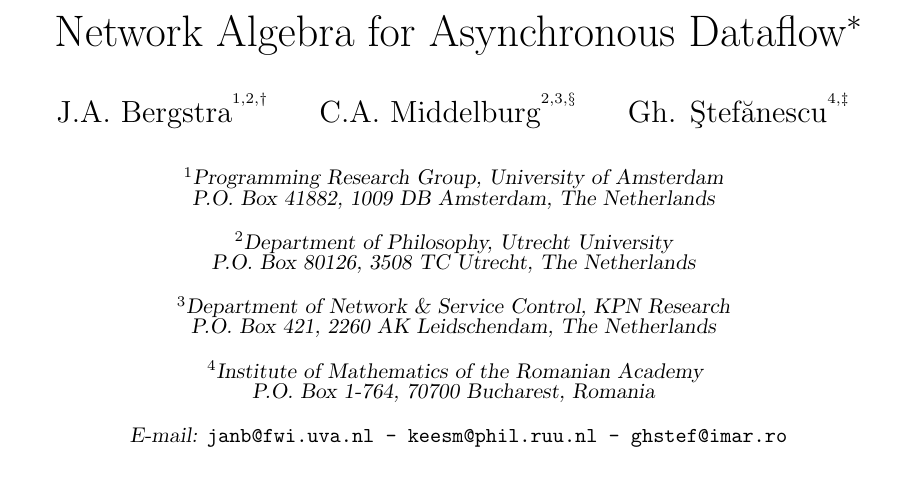
\includegraphics[width=0.9\textwidth]{Bergstra.png}}
      \end{figure}
    \end{column}
  \end{columns}
\end{frame}

\section{Isabelle/HOL Preliminaries}

\begin{frame}[fragile]
  \frametitle{Isabelle/HOL}
  \begin{itemize}
    \item Classical higher-order logic (HOL):\\ Simple Typed Lambda Calculus + axiom of choice + axiom of infinity + rank-1 polymorphism
          \pause
    \item Isabelle: A generic proof assistant
          \begin{overlayarea}{\textwidth}{.3\textheight}
            \centering
            \begin{figure}
              \centering
              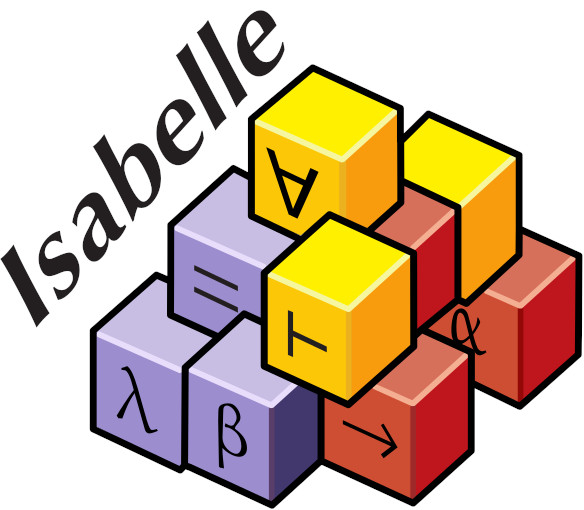
\includegraphics[scale=0.15]{isabelle}
            \end{figure}
          \end{overlayarea}
    \item Isabelle/HOL: Isabelle's flavor of HOL
  \end{itemize}
  \pause
    \begin{block}{Why Isabelle/HOL?}
      \begin{itemize}
        \item Codatatypes: (possibly) infinite data structures (e.g., lazy lists, streams)
        \item Corecursion: always eventually produces some codatatype constructor
        \item Coinductive predicate: infinite number of introduction rule applications
        \item Coinduction: reason about coinductive predicates
      \end{itemize}
  \end{block}

\end{frame}

\section{Operators as a Codatatype}

\begin{frame}[fragile]
  \frametitle{Operators}
  \begin{itemize}
    \item Codatatypes
          \vspace*{-1ex}
  \end{itemize}
\end{frame}

\begin{frame}[fragile]
  \frametitle{Examples}
  \begin{itemize}
    \item Codatatypes
          \vspace*{-1ex}
  \end{itemize}
\end{frame}

\begin{frame}[fragile]
  \frametitle{Operators Equivalences: Motivation}
  \begin{itemize}
    \item foo
  \end{itemize}
\end{frame}

\begin{frame}[fragile]
  \frametitle{Operators Equivalences: Strong Bisimilarity}
  \begin{itemize}
    \item foo
  \end{itemize}
\end{frame}

\begin{frame}[fragile]
  \frametitle{Operators Equivalences: Weak Bisimilarity}
  \begin{itemize}
    \item foo
  \end{itemize}
\end{frame}

% \begin{frame}[fragile]
%   \frametitle{Operators Equivalences: Trace Equivalence}
%   \begin{itemize}
            %       \item foo
            %     \end{itemize}
            %             \end{frame}

            %             \begin{frame}[fragile]
            %             \frametitle{Numeral Types for Ports}
            %             \begin{itemize}
            %       \item foo
            %     \end{itemize}
            %             \end{frame}

\section{Asynchronous Dataflow Operators}

\begin{frame}[fragile]
  \frametitle{Buffer Infrastructure}
  \begin{itemize}
    \item foo
  \end{itemize}
\end{frame}

\section{Asynchronous Dataflow Properties}

\section{Conclusion}

\begin{frame}
  \frametitle{Conclusion}
  \begin{itemize}
    \item Isabelle/HOL has a good tool set to formalize and reason about stream processing:
          \begin{itemize}
            \item Codatatypes, coinductive predicates, corecursion with friends, reasoning up to friends (congruence),
                  \begin{itemize}
                    \item Coinduction up to congruence principle is automatically derived for codatatypes (but not for coinductive principles)
                  \end{itemize}
          \end{itemize}
    \item Next step: Feedback loop
  \end{itemize}
\end{frame}
            %             slide about tecnicques used, coinduction principles, friends, reasoning up to friends, generalization using skip_op, combining coinduction and induction, coinduction up to congruence for coinductive predicates, say our paper is more detailed in these topics

\section{Questions, comments and suggestions}

\end{document}
